\section{Relevance}\label{sec:relevance}

Chess has been a popular game since its start and introduction in the western world.
It would not be an overstatement to say that it is one of the most recognizable and popular games in the world, being
one of the favorite games of children and adults alike.
Chess is even played in Danish schools through the non-profit \textit{Skoleskak} initiative~\cite{skoleskak2024}.
On top of the already existent popularity, the game of chess has risen in popularity and quite literally taken
the world by storm in recent years.

In the following section, we will briefly examine some influences and reasons why chess has seen such an almost
unprecedented increase in popularity in recent years.
We will also explore the benefits of teaching and playing chess, and how the popularity increase of the game translates
into a potential market opportunity.
In summary, we will present the societal relevance of creating an online chess learning application.

\subsection{Increasing popularity}\label{subsec:increasing-popularity}

The rise in popularity can, e.g., be seen in the growth in Google searches for the keyword \textit{chess} in the last 5
years, as can be seen in Figure~\ref{fig:google-trends}.
\textit{Chess} searches doubled in late 2020, after which they stagnated.
Despite the stagnation, the current search volume is still double what it was 4 years ago at the beginning of the new
chess craze.

% textidote: ignore begin % For some reason (probably bug), `sh:capperiod` is wrongly emitted in the caption.
\begin{figure}
    \centering
    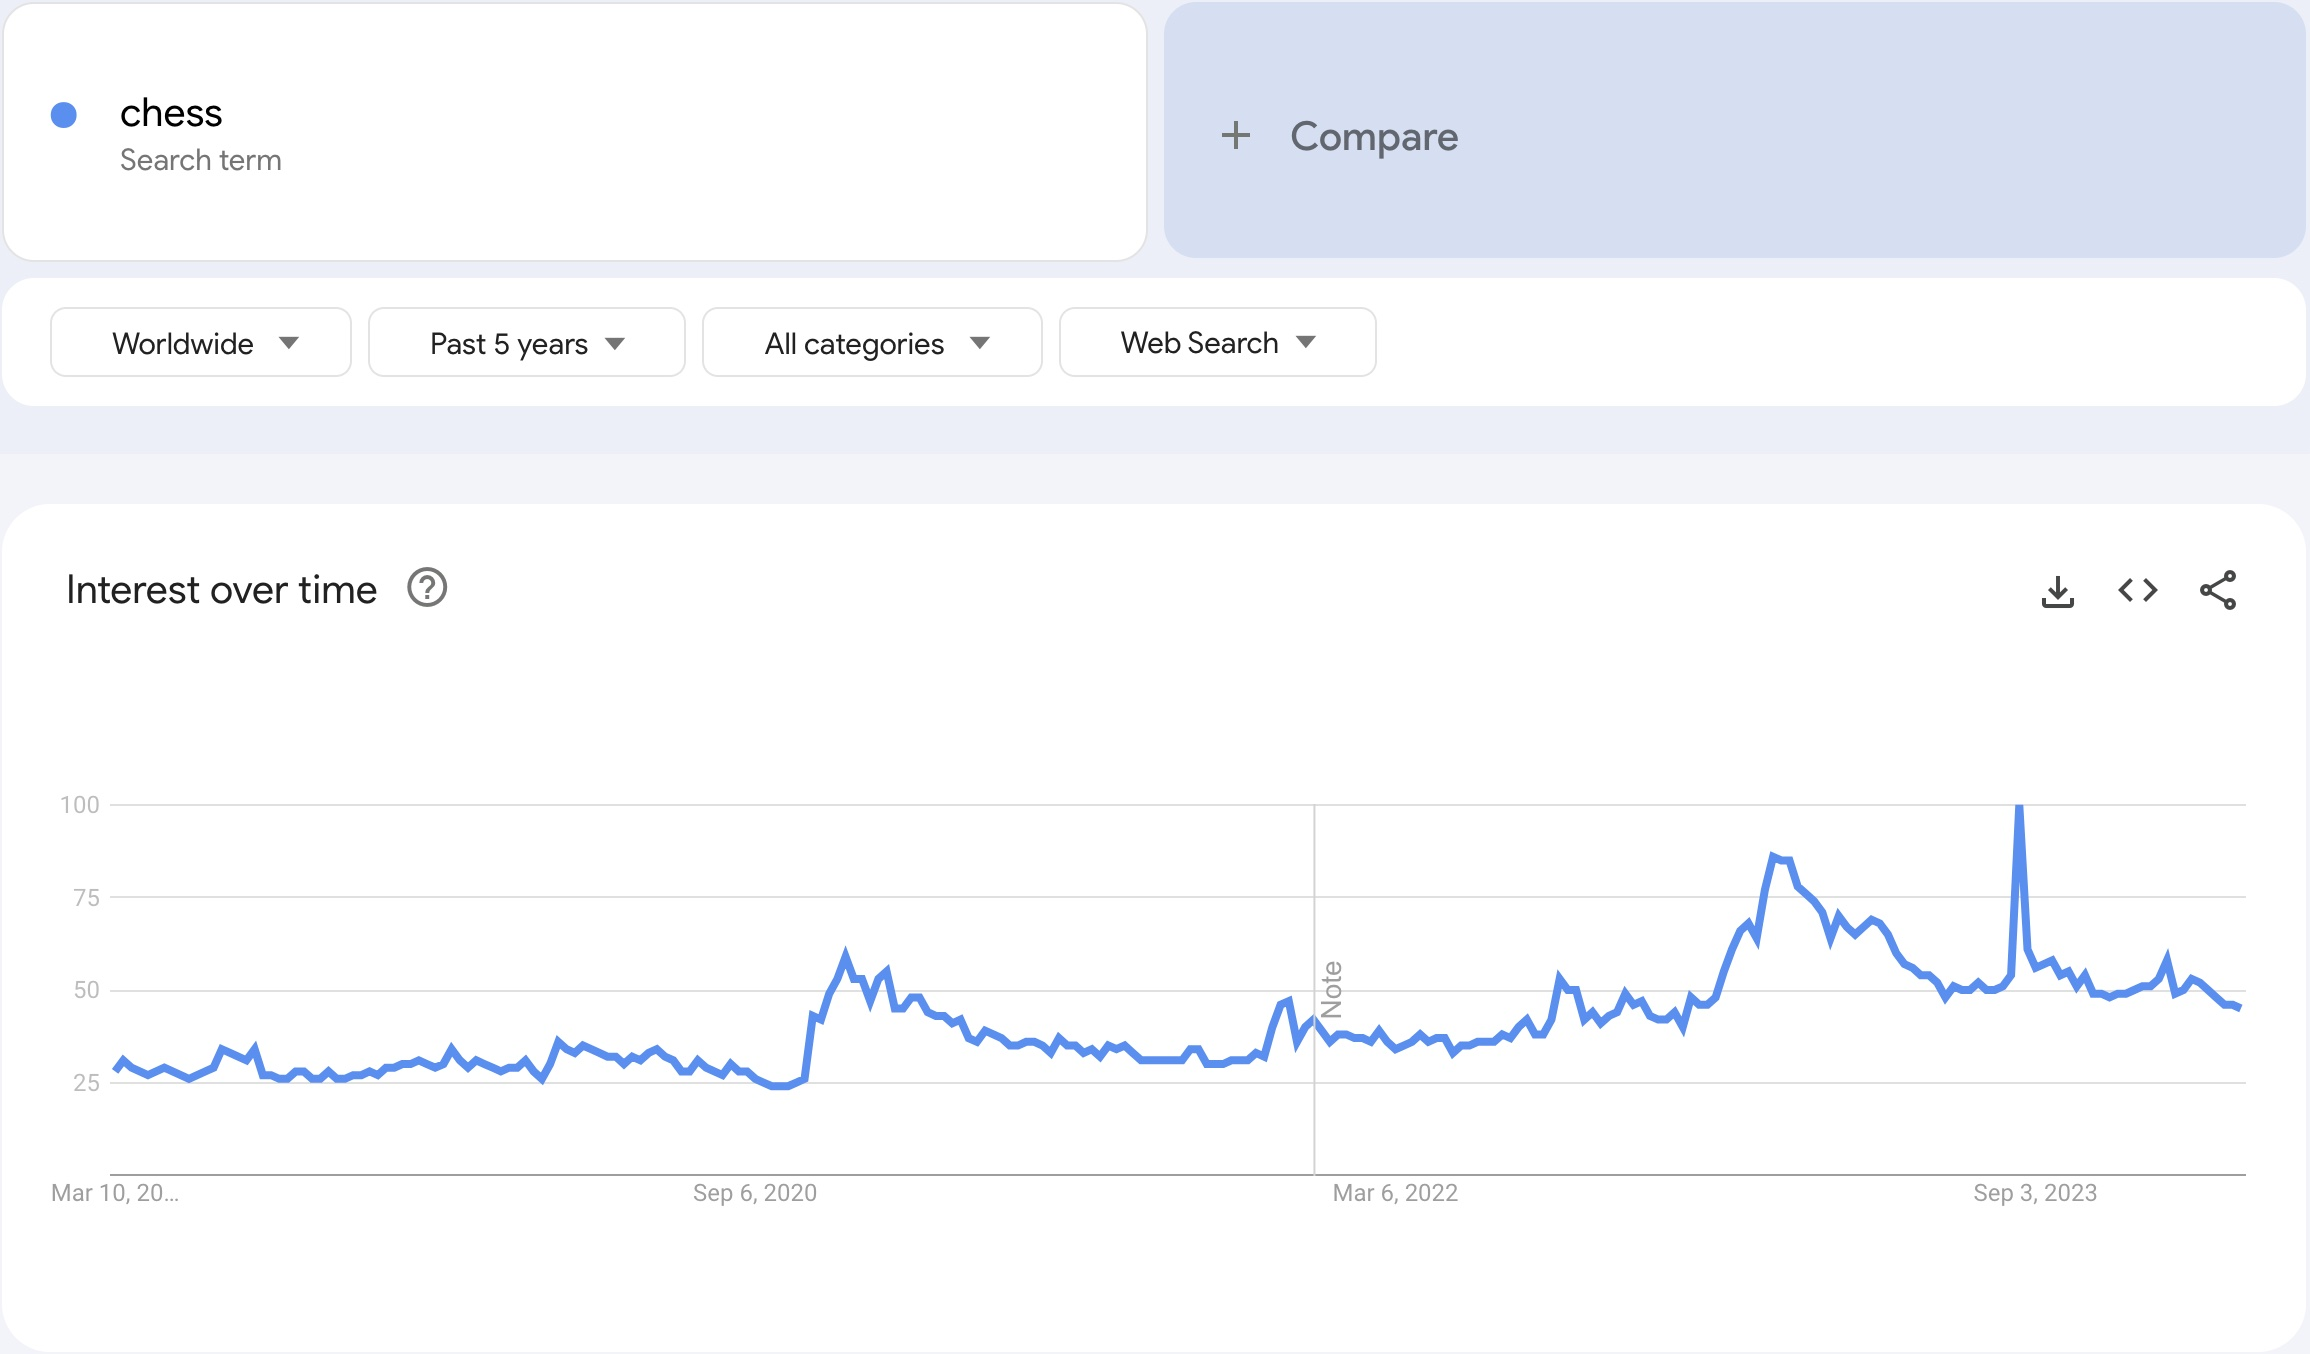
\includegraphics[width=0.8\textwidth]{google-trends}
    \caption{Google Trends result for the keyword \textcquote{google-trends2024}{chess}.}\label{fig:google-trends}
\end{figure}
% textidote: ignore end

One of the primary factors in the recent raise in popularity can be attributed to the COVID-19 pandemic that broke out
in March 2020.
Isolated at home and in need of entertainment, cognition, or social activities, many people turned to online activities
in search for suitable new skills to learn or things to occupy their time with~\cite{nyt2022}.
% textidote: ignore begin % Due to `sh:d:002` on `\verb|Chess.com|`
During this period,~\verb|Chess.com|, one of the main \textit{players} in the chess world, saw its user base more than
double.
% textidote: ignore end
% textidote: ignore begin % Due to `sh:d:002` on `Chess.com`
As The New York Times writes:~\textcquote{nyt2022}{From October 2020 to April 2022, Chess.com saw their number of
monthly active users double from roughly 8 million to nearly 17 million}.
% textidote: ignore end

This rapid increase in players and potential players was further amplified by the release of the show ``The Queen's
Gambit'', which was an international success, attracting 62 million viewers in the first month of its
release~\cite{deadline2020}.
Looking again at Figure~\ref{fig:google-trends}, the first spike in growth, around September 2020, coincides with the
release of the series~\cite{nyt2022}.
This show, through the simple-to-understand medium of a TV show, inspired a large audience to pick up chess-playing as
an activity~\cite{polygon2023}.
Chess went mainstream, so to speak.

\subsection{Benefits}\label{subsec:benefits}

Chess is not only a game, but is also known for being excellent in a lot of health- and life-related aspects.
% textidote: ignore begin % Due to the quote having odd grammar.
As Benjamin Franklin wrote:~\blockcquote{franklin1786}{``The game of Chess is not merely an idle amusement. Several very
valuable qualities of the mind, useful in the course of human life, are to be acquired or strengthened by it, so as to
become habits, ready on all occasions. For life is a kind of chess, in which we have often points to gain, and
competitors or adversaries to contend with, and in which there is a vast variety of good and ill events, that are, in
some degree, the effects of prudence or the want of it''}.
% textidote: ignore end

As the quote outlines, chess can have benefits far beyond just being a source of entertainment.

Long-term chess-playing has been shown to increase auditory memory function~\cite{fattahi2015}.
Another analysis that explored the benefits of regular chess playing among schoolchildren suggests that chess improves
cognitive and problem-solving skills, and enriches social-emotional development~\cite{aciego2012}.
To add on to that, a third study~\textcquote{poston2019}{statistically shows that learning chess increases a
student's academic performance}.
This study further explains, even more interestingly, that the benefits of learning chess are proportional to the skill
level of the player, i.e., the better you are at the game, the more your brain gains from the gameplay.

\subsection{A new market}\label{subsec:a-new-market}

And finally, especially chess as an online game presents itself as an excellent new business market with a lot of
potential~\cite{business-insider2021}.
In a study conducted by AGON in 2012, the company responsible for organizing and hosting the chess events by FIDE (The
International Chess Federation), an estimated 605 million adults play chess regularly~\cite{chessbase2012}.

In response to its growing popularity, the esports industry has taken notice of chess as a potentially lucrative
investment opportunity.
Esports organizations, who traditionally focused on and invested in young players from the more traditional video game
scene, have begun to recognize the strategic depth and entertainment value of chess.
As a result, a wave of signings and partnerships between esports teams and prominent chess professionals and content
creators has been seen in the last couple of years.
Most notably~\textcquote{business-insider2021}{the esports team TSM signed the five-time US chess champion and streamer
Hikaru Nakamura}.
These collaborations signal a significant shift in the perception of chess within the broader esports ecosystem,
positioning it as a viable and exciting addition to the competitive gaming landscape.

% TODO Make this subsection longer, and remove the TeXtidote ignore comments
% textidote: ignore begin

\subsection{Conclusion}\label{subsec:conclusion}
% textidote: ignore end

In conclusion, the recent surge in popularity of chess signifies a remarkable evolution in the game's cultural
significance and potential.
Moreover, the rise of online platforms and streaming services has democratized access to the game, enabling individuals
to participate in competitive play and educational activities from the comfort of their homes.

Beyond its entertainment value, chess offers a wide array of cognitive, social, and academic benefits, making it an
invaluable tool for personal development and education.

Overall, the societal relevance of creating an online chess learning application lies in its ability to capitalize on
the growing popularity of chess, while also providing a platform for education, engagement, and innovation within the
game.
